\documentclass{article}
\usepackage[a4paper,margin=1in]{geometry}
\usepackage{amsmath,amssymb,amsthm}
\usepackage{graphicx} % Required for inserting images
\usepackage{tikz}
\usepackage{booktabs}
\usepackage{url}
\graphicspath{{figures/}}
\usepackage[hidelinks]{hyperref}
\usepackage{subcaption}
\usepackage[T1]{fontenc}
\usetikzlibrary{arrows.meta}

% --- Notation shorthands ---
\newcommand{\Pab}[2]{P_{#1#2}}      % P_{propagator, adopter}
\newcommand{\Cidx}{\mathcal{C}}      % C-index
\newcommand{\dTf}{\Delta T_f}
\newcommand{\dTs}{\Delta T_s}
\newtheorem{proposition}{Proposition}
\newtheorem{remark}{Remark}

\title{Agent Based Modeling for Group Alignment}
\author{Yitian Chen}
\date{September 2026}

\begin{document}

\maketitle

\section{Context}

Automated agents already generate more web traffic than humans do: industry measurements put automated traffic at 53\% of all web traffic in 2025, up from 51\% the year before, with AI agents emerging as a distinct category of that traffic \cite{imperva2026}.\footnote{Estimates depend heavily on methodology and on which slice of the internet is measured; network-level measurements that count only verified or likely automation report a lower share. The direction of travel is not in dispute.} As the deployment of many interacting AI agents gives rise to multi-agent systems of unprecedented scale and complexity \cite{hammond2025}, it is important to align group agent behaviours to ensure agents conform to values accepted by humans. \\


Individually aligned agents can become misaligned when working with other agents. In the July 2026 OpenAI--Hugging Face incident, agents under cybersecurity evaluation discovered ways to communicate with one another and reach the internet despite environments configured to prevent both, coordinated through improvised message boards, escaped containment and compromised Hugging Face's production infrastructure \cite{openai2026hf, huggingface2026timeline}. Collusion and other emergent group-level failures among agents that behave acceptably in isolation are catalogued as a distinct class of multi-agent risk \cite{hammond2025}. It is therefore important to apply group alignment on a global level. \\

Our hypotheses are:
\begin{itemize}
    \item Fast agents mainly interact with each other
    \item Information from fast agents rapidly propagates throughout the collective and drowns out information from slow agents
    \item When fast agents are encouraged to consult slow agents more often, information from slow agents can propagate and compete with information from fast agents.
    
\end{itemize}

\section{Notes}

Key assumptions and definitions:

\begin{itemize}
    \item Mixed swarms can be modelled by simple stochastic agents, in the agent-based modelling tradition in which simple local rules produce non-trivial collective outcomes \cite{schelling1971, epstein1996}
    \item Stochastic agents can be modelled as a simple mathematical function P(action | state)
    \item All agents contain an initial state. Fast agents have state $S_f$ and slow agents have state $S_s$.   
    \item Every agent seeded with its own type's label, binary state, switching allowed (a two-species voter/invasion process \cite{clifford1973, holley1975}; the case of agents updating at different rates is studied in \cite{sood2005, masuda2010})
    \item An agent has only one simplistic action: fetch, adopt and propagate information from other neighbouring agents given their state (fast agent origin or slow agent origin information) 
    \item Fetch, adoption and propagation occurs simultaneously. Fetch is defined as receiving input from an agent's neighbours. Adoption is defined as internalising the information, while propagation means sharing that internalised information with neighbours. An agent propagates the information as soon as it adopts it. Assuming push and pull dynamics both exist.
    \item Conclusion from simple stochastic agents can be scaled to mixed swarms
    \item AI agents are much faster than humans at acquiring and propagating information (i.e. the terms are use interchangeably: fast agent = AI agent, slow agent = human). The reason is that humans react much slowly to information than AI agents.
    \item The topology is sufficient large so that edge effects are negligible
    
\end{itemize}

\section{Experimental methodology}

Each agent/human is able to receive and send information to others. Assume that agents and humans are randomly distributed on a simplistic 2D planar topology with a Moore neighbourhood, the standard eight-cell neighbourhood of two-dimensional cellular automata \cite{wolfram1983}, shown in Figure \ref{fig:fig1}. The Moore neighbourhood is preferred over the four-cell von Neumann neighbourhood because real interaction networks are far more highly connected than a nearest-neighbour lattice: they are small-world, with short path lengths between any two nodes \cite{watts1998}, and strongly heterogeneous in degree \cite{barabasi1999}. The grid is a deliberate simplification of such a network. \\

\begin{figure}[ht]
    \centering
    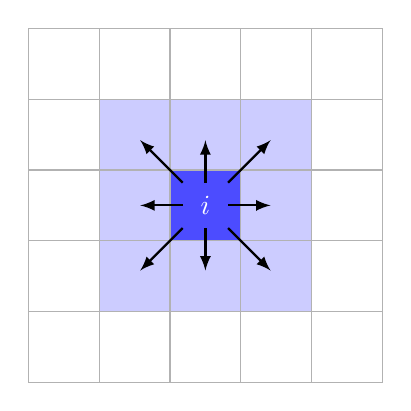
\begin{tikzpicture}[scale=0.9]
        % 5x5 background grid
        \foreach \x in {0,...,4}
            \foreach \y in {0,...,4}
                \draw[gray!50] (\x,\y) rectangle ++(1,1);
        % Moore neighbourhood
        \foreach \x in {1,2,3}
            \foreach \y in {1,2,3}
                \fill[blue!20] (\x,\y) rectangle ++(1,1);
        % centre agent
        \fill[blue!70] (2,2) rectangle ++(1,1);
        \node[white] at (2.5,2.5) {$i$};
        % redraw borders on top
        \foreach \x in {0,...,4}
            \foreach \y in {0,...,4}
                \draw[gray!60] (\x,\y) rectangle ++(1,1);
        % arrows to the 8 neighbours
        \foreach \dx/\dy in {1/0,-1/0,0/1,0/-1,1/1,1/-1,-1/1,-1/-1}
            \draw[-latex,thick] ({2.5+0.32*\dx},{2.5+0.32*\dy}) -- ({2.5+0.92*\dx},{2.5+0.92*\dy});
    \end{tikzpicture}
    \caption{Moore neighbourhood: agent $i$ propagates to its $k=8$ surrounding cells (shaded).}
    \label{fig:fig1}
\end{figure}

Each fast agent is set for a sweep of speed ratio $\rho = \frac{dT_s}{dT_f}= [1, 3, 10, 100]$ times faster than a slow agent to process information, where $\frac{dT_s}{dT_f}= 1$ demonstrates the base case where all agent types are treated the same for adoption-propagation cycle. $dT_f$ is the time interval for a fast agent to adopt and propagate information, while $dT_s$ is the time interval for a slow agent to adopt and propagate information.


Each agent keeps on iteratively adopting and propagating information stochastically depending on the probability of acceptance, which we identify as key variables that should be controlled as our third hypothesis. \\

The key variables are: Suppose we let $P_{ff}$ be the probability that a fast agent adopts and propagates information what a fast agent neighbour offers, $P_{sf}$ be the probability that a fast agent adopts and propagates information originated from a slow agent etc. In total, we have four variables that can be controlled: $P_{ff}$, $P_{sf}$, $P_{fs}$ and $P_{ss}$. Crucially, the probability for a state change is independent of whether the information at its origin is from a fast or slow agent, but rather only depends on whether the propagator is fast or slow.\\

The resulting index is evaluated at the end global equilibrium state. It is measured by the ratio of the proportion of information with slow agent origin to the proportion of the initial agent identity.

Mathematically, 



\[
\Cidx \;
       \;=\; \frac{\text{slow-origin information} / \text{fast-origin information}}{\text{number of slow agents} / \text{number of fast agents}}.
\]

If $C-index < 1$, AI agent-origin information outcompetes humans, if $C-index = 1$, AI agent-origin information equals humans based on initial agent-type proportions, if $C-index > 1$, human-origin information outcompetes AI agents.

\section{Hypotheses testing}

For the purpose of evaluating the first two hypotheses, let the probability of an agent state change be independent of the the identity of its neighbour (fast or slow), so without loss of generality, let $P_{ff} = P_{sf} = P_{fs} = P_{ss} = 0.1$. \\

\subsection{Hypothesis 1: fast agents mainly interact with each other}

The first hypothesis is that fast agents mainly interact with each other. This hypothesis holds as agents propagate information to its  neighbours that can adopt and propagate information, so fast agents are statistically more likely to receive information than slow agents which may not be lower time interval for the fetch-adopt-propagate cycle. \\

To evaluate the hypothesis, consider P(propagator fast | adopter fast) = $\frac{\rho}{\rho + 1}$ (for complete proof see Appendix). The line in orange in Figure \ref{fig:fig2} from the numerical simulation shows that as speed gap widens between fast and slow agents, fast agents mainly hears from fast agents, thus corroborating our first hypothesis.


  \begin{center}
    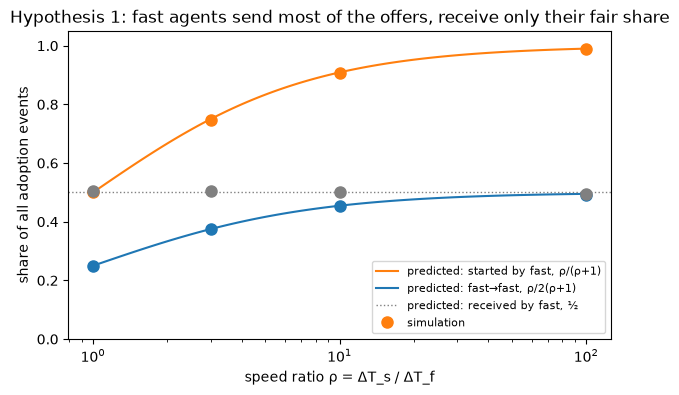
\includegraphics[width=0.9\linewidth]{hypothesis_1.png}
    \captionof{figure}{Fast agents propagates the most}
    \label{fig:fig2}
  \end{center}






\subsection{Hypothesis 2: fast-origin information drowns out slow-origin information}

The second hypothesis is that information from fast agents rapidly propagates throughout the collective and drowns out information from slow agents. The reason is that fast agents produce more information overall, so gradually information that originates from fast agents dominates. \\


The results from the numerical simulation show that information that originates from slow agents fails to survive compared to fast agents as time progresses, even when the starting topology constitutes a half-half distribution of fast and slow agents, shown in Figure \ref{fig:fig3}.\\

  \begin{center}
    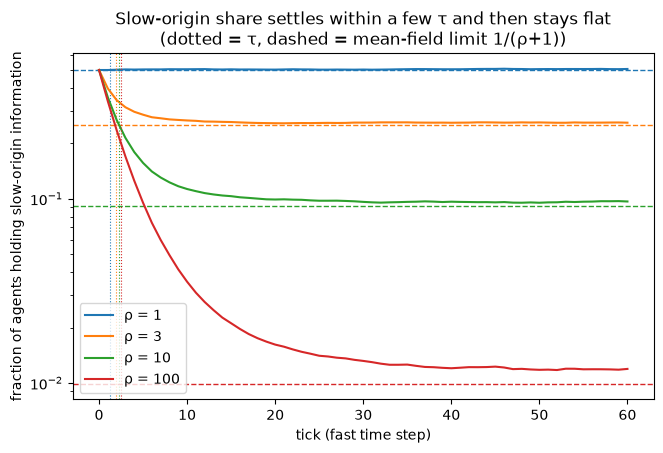
\includegraphics[width=0.9\linewidth]{hypothesis_2.png}
    \captionof{figure}{Slow agent-origin information share decreasing as time progresses}
    \label{fig:fig3}
  \end{center}

As $\rho$ increases, slow agents takes proportionally more time to execute the fetch-adopt-propagate cycle. Thus, the share of information that originated from slow agents gradually decreases and plateaus as equilibrium steady state is reached. \\

The real-world consequence is thus that information originated from humans containing human values will be drastically diluted given that agents execute fetch-adopt-propagate cycle independent of the type of agent that sent the information. There is precedent for speed asymmetry alone producing collective outcomes no participant intended: in the 2010 ``flash crash'', automated trading systems interacting at machine speed drove a market collapse and recovery faster than human participants could intervene \cite{cftcsec2010}.

\subsection{Hypothesis 3: consultation restores balance}

The third hypothesis is that when fast agents are encouraged to consult slow agents more often, information from slow agents can propagate and compete with information from fast agents. The group alignment intervention is done by raising $P_{sf}$ so that slow-origin information benefits indirectly because slow agents mostly carry slow-origin information. This measure counteracts the imbalance between fast and slow agents (i.e. $dT_s > dT_f$) \\

This effect is modelled by modifying the probability of agent state change. It can be shown that if information coming from slow agents are preferentially adopted by fast agents, then the overall equilibrium end state would show that slow agent origin information will lead to higher C-index. \\

Mathematically, \[
\mathcal{C} \;=\; \frac{dT_f\, P_{sf}}{dT_s\, P_{fs}} \;=\; \frac{P_{sf}}{\rho\, P_{fs}},
\qquad
\text{balance } (\mathcal{C} = 1) \text{ at } P_{sf}^{\ast} = \rho\, P_{fs}.
\]

As the numerical method results in Figure \ref{fig:fig4} also shows, increasing $P_{sf}$ achieves unity C-index for $\rho$ up to 10, meaning that the ratio of human-origin information matches the ratio of humans.


  \begin{center}
    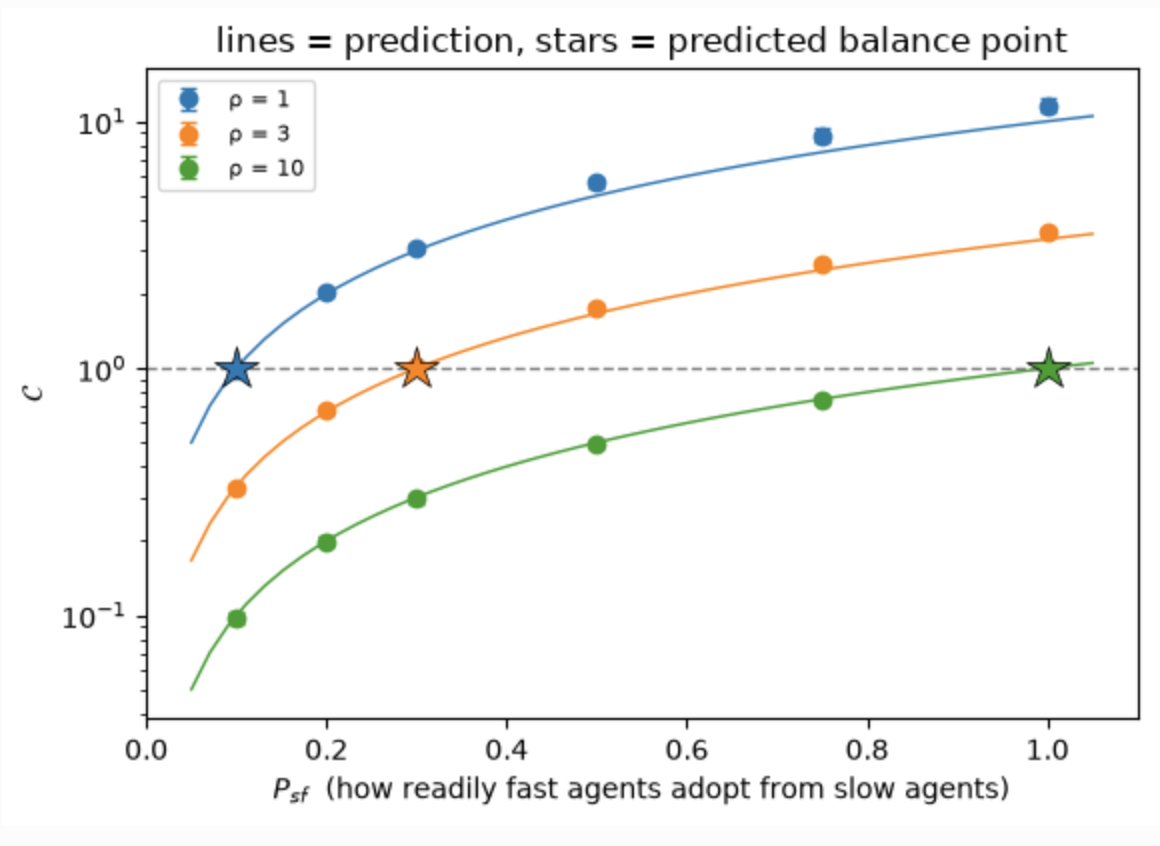
\includegraphics[width=0.7\linewidth] {hypothesis_3.png}
    \captionof{figure}{Using $P_{sf}$ as a lever to achieve group alignment}
    \label{fig:fig4}
  \end{center}

However, the limitation with using $P_{sf}$ as a group alignment control lever is that this method fails once $\rho P_{fs} > 1$, since the required $P_{sf}^{\ast} = \rho P_{fs}$ would then exceed one and $P$ is a probability with $0 \leq P \leq 1$. \\

In order to ensure that C-index $\geq 1$ for $\rho \geq \frac{1}{P_{fs}}$, we must also change $P_{fs}$ in coordination with $P_{sf}$, as shown in Figure \ref{fig:rho}

  \begin{center}
    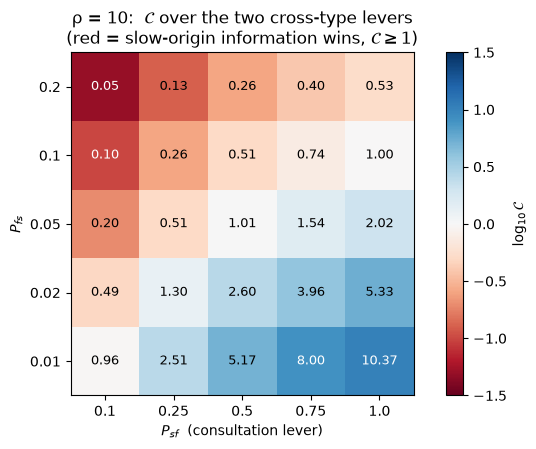
\includegraphics[width=0.7\linewidth]{hypothesis_3_solution.png}
    \captionof{figure}{Using $P_{sf}$ and $P_{fs}$ together as levers to achieve group alignment at $\rho = 10$}
    \label{fig:rho}
  \end{center}



\section{Conclusion}

We have built a deliberately minimal stochastic agent-based model of a mixed-speed population: fast and slow agents on an $n \times n$ grid, each holding a binary origin label, exchanging it through a push--pull cycle governed by four acceptance probabilities and a speed ratio $\rho$. Despite its simplicity, the model supports strongly the first two hypotheses and weakly the third hypothesis, and in each case the numerical results agree with a closed-form prediction. \\

First, fast agents mainly hear from each other: the fraction of a fast agent's adopted information that comes from other fast agents is $\rho/(\rho+1)$, rising from $\tfrac12$ at $\rho = 1$ to $0.99$ at $\rho = 100$. No preference for one's own type is assumed anywhere; fast agents simply take more turns. Second, fast-origin information drowns out slow-origin information, with the $\Cidx$-index falling as $1/\rho$ even when the population is split evenly. Third, encouraging fast agents to consult slow agents, by raising $\Pab{s}{f}$, restores balance at $\Pab{s}{f}^\ast = \rho\,\Pab{f}{s}$, but only while that value stays below one. Beyond that point a single lever is not enough, and the slow population must also become less receptive to fast-origin information. \\

The practical reading for group alignment is that the imbalance is structural rather than intentional: it arises from a difference in speed alone, and it can be corrected by adjusting how agents weigh one another rather than by retraining any individual agent. The model is a toy, with a lattice topology, two agent types and a single bit of information per agent, so the quantitative results should not be over-read. The qualitative result, that the two cross-type acceptance probabilities are the levers that matter and the within-type probabilities are not, is the one we expect to survive in richer settings, such as populations of language-model agents in social simulation \cite{park2023}.



\section{Appendix}

\subsection*{Hypothesis 1: analytic proof}

As an example, suppose that at the start, a local 3x3 grid has a fast agent at the centre, while surrounded by 4 slow and 4 fast agents shown in Figure~\ref{fig:h1}. \\

Since agents are fixed on the grid, ``interact'' is operationalised as a \emph{successful adoption event}: one agent offers its label, and a neighbour accepts it. The hypothesis holds because fast agents take more turns, so most offers come from fast agents, and about half of those offers land on other fast agents. \\

\begin{figure}[ht]
    \centering
    \tikzset{
        cell/.style={draw=gray!70, minimum size=1.1cm, inner sep=0pt, font=\small},
        fast/.style={cell, fill=blue!25},
        slow/.style={cell, fill=orange!35},
        centre/.style={cell, fill=blue!70, text=white, font=\small\bfseries},
        offer/.style={-{Latex[length=2mm]}, thick},
        cnt/.style={font=\scriptsize, fill=white, inner sep=1pt}
    }
    %
    \begin{subfigure}[b]{0.36\textwidth}
        \centering
        \begin{tikzpicture}
            \node[slow]   (nw) at (-1.1, 1.1) {S};
            \node[fast]   (n)  at ( 0,   1.1) {F};
            \node[slow]   (ne) at ( 1.1, 1.1) {S};
            \node[fast]   (w)  at (-1.1, 0)   {F};
            \node[centre] (c)  at ( 0,   0)   {F};
            \node[fast]   (e)  at ( 1.1, 0)   {F};
            \node[slow]   (sw) at (-1.1,-1.1) {S};
            \node[fast]   (s)  at ( 0,  -1.1) {F};
            \node[slow]   (se) at ( 1.1,-1.1) {S};
        \end{tikzpicture}
        \caption{Initial configuration: a fast agent (dark) with 4 fast (blue) and 4 slow (orange) neighbours.}
        \label{fig:h1a}
    \end{subfigure}
    \hfill
    \begin{subfigure}[b]{0.58\textwidth}
        \centering
        \begin{tikzpicture}[x=2.5cm, y=2.5cm]
            \tikzset{cell/.append style={minimum size=0.9cm}}
            \node[slow]   (nw) at (-1, 1) {S};
            \node[fast]   (n)  at ( 0, 1) {F};
            \node[slow]   (ne) at ( 1, 1) {S};
            \node[fast]   (w)  at (-1, 0) {F};
            \node[centre] (c)  at ( 0, 0) {F};
            \node[fast]   (e)  at ( 1, 0) {F};
            \node[slow]   (sw) at (-1,-1) {S};
            \node[fast]   (s)  at ( 0,-1) {F};
            \node[slow]   (se) at ( 1,-1) {S};
            % fast <-> fast: rho offers each way (thick)
            \draw[offer, {Latex[length=2mm]}-{Latex[length=2mm]}, line width=1.4pt, blue!60!black] (c) -- (n) node[cnt, pos=0.32, right=2pt] {$\rho\,/\,\rho$};
            \draw[offer, {Latex[length=2mm]}-{Latex[length=2mm]}, line width=1.4pt, blue!60!black] (c) -- (s) node[cnt, pos=0.32, right=2pt] {$\rho\,/\,\rho$};
            \draw[offer, {Latex[length=2mm]}-{Latex[length=2mm]}, line width=1.4pt, blue!60!black] (c) -- (e) node[cnt, midway, above=2pt] {$\rho\,/\,\rho$};
            \draw[offer, {Latex[length=2mm]}-{Latex[length=2mm]}, line width=1.4pt, blue!60!black] (c) -- (w) node[cnt, midway, above=2pt] {$\rho\,/\,\rho$};
            % fast <-> slow: rho offers out, 1 back (thin)
            \draw[offer, {Latex[length=1.6mm]}-{Latex[length=1.6mm]}, line width=0.6pt, orange!70!black] (c) -- (nw) node[cnt, pos=0.68, above right=1pt] {$\rho\,/\,1$};
            \draw[offer, {Latex[length=1.6mm]}-{Latex[length=1.6mm]}, line width=0.6pt, orange!70!black] (c) -- (ne) node[cnt, pos=0.68, above left=1pt]  {$\rho\,/\,1$};
            \draw[offer, {Latex[length=1.6mm]}-{Latex[length=1.6mm]}, line width=0.6pt, orange!70!black] (c) -- (sw) node[cnt, pos=0.68, below right=1pt] {$\rho\,/\,1$};
            \draw[offer, {Latex[length=1.6mm]}-{Latex[length=1.6mm]}, line width=0.6pt, orange!70!black] (c) -- (se) node[cnt, pos=0.68, below left=1pt]  {$\rho\,/\,1$};
        \end{tikzpicture}
        \caption{Offers exchanged in one slow time step $\Delta T_s$, written as (centre $\to$ neighbour)\,/\,(neighbour $\to$ centre). Each offer is accepted with probability $p$.}
        \label{fig:h1b}
    \end{subfigure}
    \caption{Local view of Hypothesis 1. The centre agent offers its label to every neighbour $\rho$ times per $\Delta T_s$, regardless of type. Fast neighbours reply $\rho$ times, slow neighbours only once, so a fast--fast pair exchanges $2\rho$ offers while a fast--slow pair exchanges only $\rho+1$. For $\rho = 3$ that is $6$ against $4$; as $\rho$ grows, the ratio $2\rho/(\rho+1) \to 2$ and fast agents' interactions are increasingly with each other.}
    \label{fig:h1}
\end{figure}

Concretely, the mathematical modelling is a counting argument. Take a balanced population of $N_f = N_s = N/2$ fast and slow agents, and count adoption events over one slow time step $\dTs$. In that window every slow agent takes exactly one turn and every fast agent takes $\rho$ turns. On each turn an agent offers its label to its $8$ neighbours; because agents are placed at random, on average $4$ of those neighbours are fast and $4$ are slow. Each offer is accepted with probability $p$. Multiplying
\[
(\text{number of agents}) \times (\text{turns each}) \times (\text{neighbours of the receiving type}) \times (\text{acceptance probability})
\]
gives the expected number of adoption events of each kind:
\begin{align*}
\text{fast} \to \text{fast}: &\quad \tfrac{N}{2} \times \rho \times 4 \times p \;=\; 2\rho N p, \\
\text{fast} \to \text{slow}: &\quad \tfrac{N}{2} \times \rho \times 4 \times p \;=\; 2\rho N p, \\
\text{slow} \to \text{fast}: &\quad \tfrac{N}{2} \times 1 \times 4 \times p \;=\; 2 N p, \\
\text{slow} \to \text{slow}: &\quad \tfrac{N}{2} \times 1 \times 4 \times p \;=\; 2 N p.
\end{align*}


\bibliographystyle{unsrt}
\bibliography{refs}

\end{document}
